\documentclass[12pt,border=0pt]{standalone}

\usepackage[utf8]{inputenc} 
\usepackage{amssymb,amsmath}
\usepackage{tikz}
\usetikzlibrary{positioning}


\thispagestyle{empty}

\begin{document}

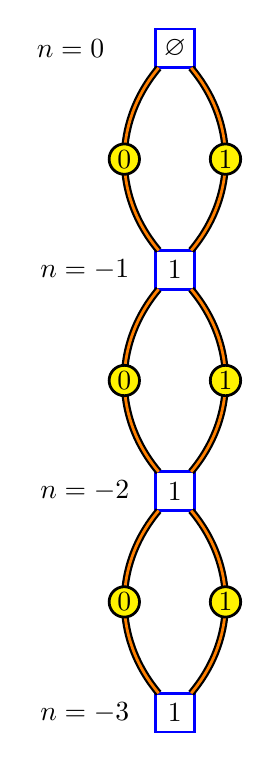
\begin{tikzpicture}[x=10pt,y=8pt]
  \centering
  \tikzset{VertexStyle/.style = {
    shape         = rectangle,
    draw          = blue, 
    fill          = white, 
  	line width    = 1pt, 
    text          = black,
    inner sep     = 1pt,
    outer sep     = 0pt,
    minimum size  = 14 pt,
    scale         = 1
    }
  }
  \tikzset{EdgeStyle/.style = {
    draw            = black, 
    thick,
    double          = orange,
    double distance = 1pt
    }
  }
  \tikzset{EdgeLabelStyle/.style = {
    draw          = black,
  	shape         = circle, 
  	line width    = 1pt, 
  	minimum size  = 10pt, 
    inner sep     = 1pt,
    outer sep     = 0pt,
    fill          = yellow,
    text          = black,
    scale         = 1
    }
  }

	\node[VertexStyle](B1) at (12.5, 35) {$\varnothing$};
	\node[VertexStyle](C1) at (12.5, 25) {$1$};
	\node[VertexStyle](D1) at (12.5, 15) {$1$};
	\node[VertexStyle](E1) at (12.5, 5) {$1$};
	\draw[EdgeStyle, bend left=-40](B1) to node[EdgeLabelStyle]{$0$} (C1);
	\draw[EdgeStyle, bend left=40](B1) to node[EdgeLabelStyle]{$1$} (C1);
	\draw[EdgeStyle, bend left=-40](C1) to node[EdgeLabelStyle]{$0$} (D1);
	\draw[EdgeStyle, bend left=40](C1) to node[EdgeLabelStyle]{$1$} (D1);
	\draw[EdgeStyle, bend left=-40](D1) to node[EdgeLabelStyle]{$0$} (E1);
	\draw[EdgeStyle, bend left=40](D1) to node[EdgeLabelStyle]{$1$} (E1);
	
	\node[left=15pt of B1]{$n=0$};
	\node[left=6pt of C1]{$n=-1$};
	\node[left=6pt of D1]{$n=-2$};
	\node[left=6pt of E1]{$n=-3$};
	
  \end{tikzpicture}

\end{document}
